\section{Sprint Backlogs}\label{sec:backlog}

In this section we will show the sprint backlogs and sprint burndown charts for every sprint so far, focusing on one sprint at a time.

\begin{figure}[H]
	\centering
	\graphicspath{ {./graphics/} }
    \centerline{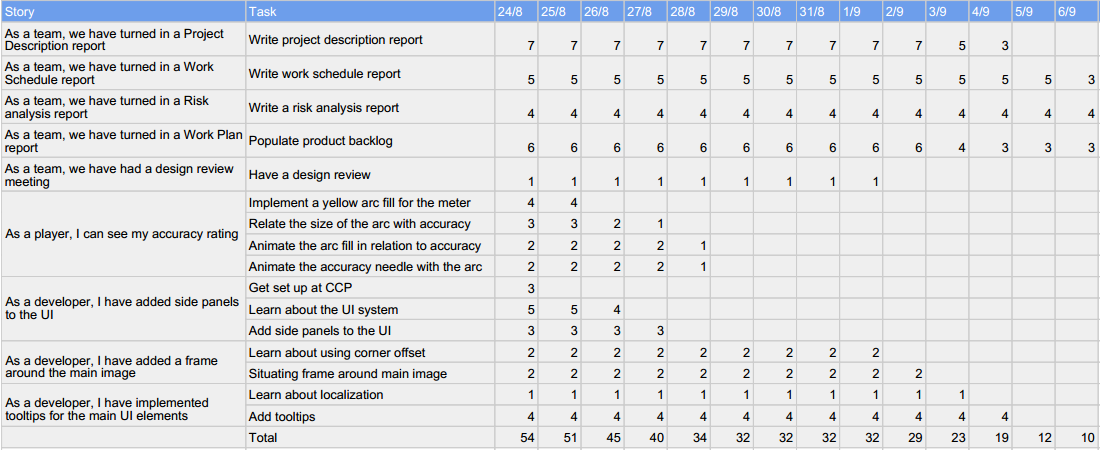
\includegraphics[scale=0.65]{sprint1.PNG}}
    \caption{\label{fig:s1}Sprint backlog for sprint 1}
\end{figure}

\begin{figure}[H]
	\centering
	\graphicspath{ {./graphics/} }
    \centerline{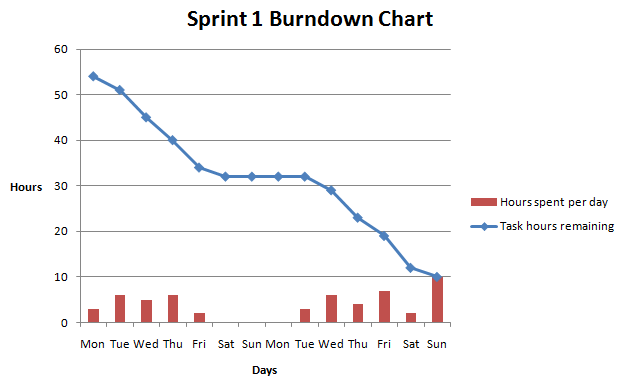
\includegraphics[scale=0.8]{sprint1bdc.PNG}}
    \caption{\label{fig:s1bd}Sprint burndown chart for sprint 1}
\end{figure}

\begin{figure}[H]
	\centering
	\graphicspath{ {./graphics/} }
    \centerline{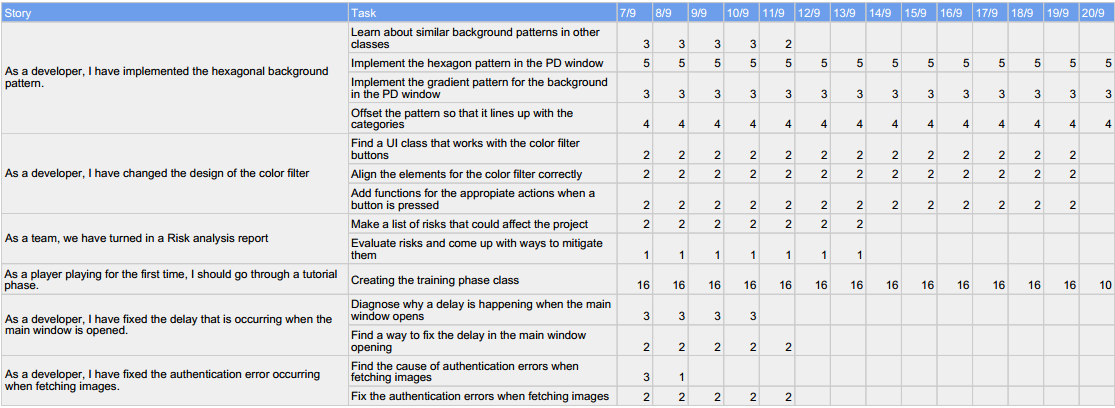
\includegraphics[scale=0.65]{sprint2.PNG}}
    \caption{\label{fig:s2}Sprint backlog for sprint 2}
\end{figure}

\begin{figure}[H]
	\centering
	\graphicspath{ {./graphics/} }
    \centerline{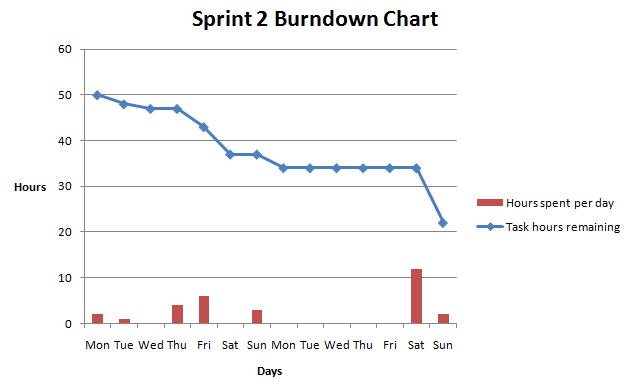
\includegraphics[scale=0.8]{sprint2bdc.PNG}}
    \caption{\label{fig:s2bd}Sprint burndown chart for sprint 2. The reason for no hours registered during the weekdays of the second week is that we used all our time on re-writing reports and preparing for the first status meeting.}
\end{figure}

\begin{figure}[H]
	\centering
	\graphicspath{ {./graphics/} }
    \centerline{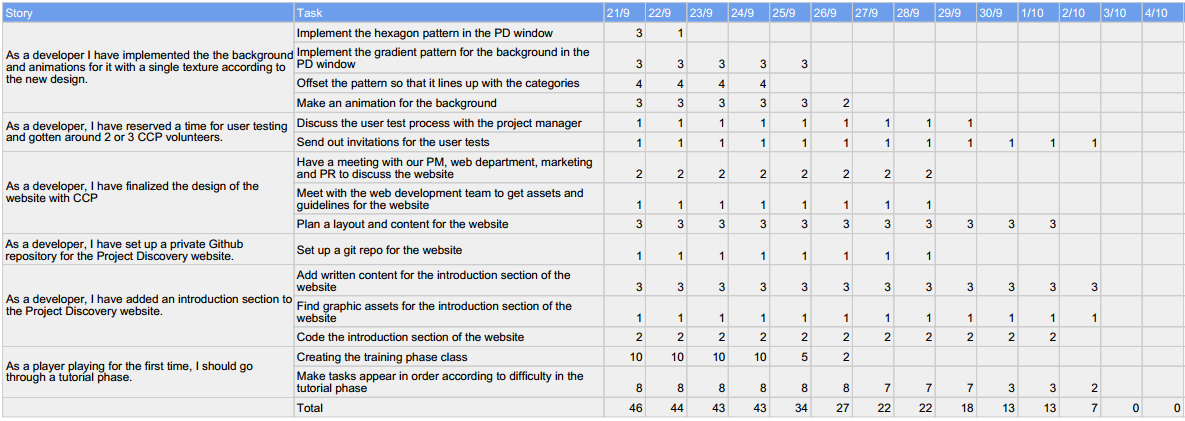
\includegraphics[scale=0.65]{sprint3.PNG}}
    \caption{\label{fig:s3}Sprint backlog for sprint 3}
\end{figure}

\begin{figure}[H]
	\centering
	\graphicspath{ {./graphics/} }
    \centerline{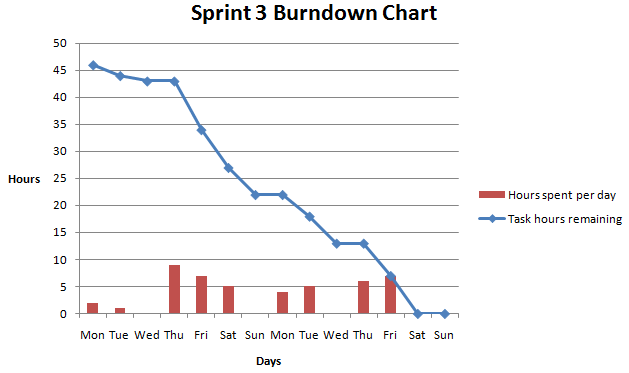
\includegraphics[scale=0.8]{sprint3bdc.PNG}}
    \caption{\label{fig:s3bd}Sprint burndown chart for sprint 3}
\end{figure}

\begin{landscape}

\begin{figure}[H]
	\centering
	\graphicspath{ {./graphics/} }
    \centerline{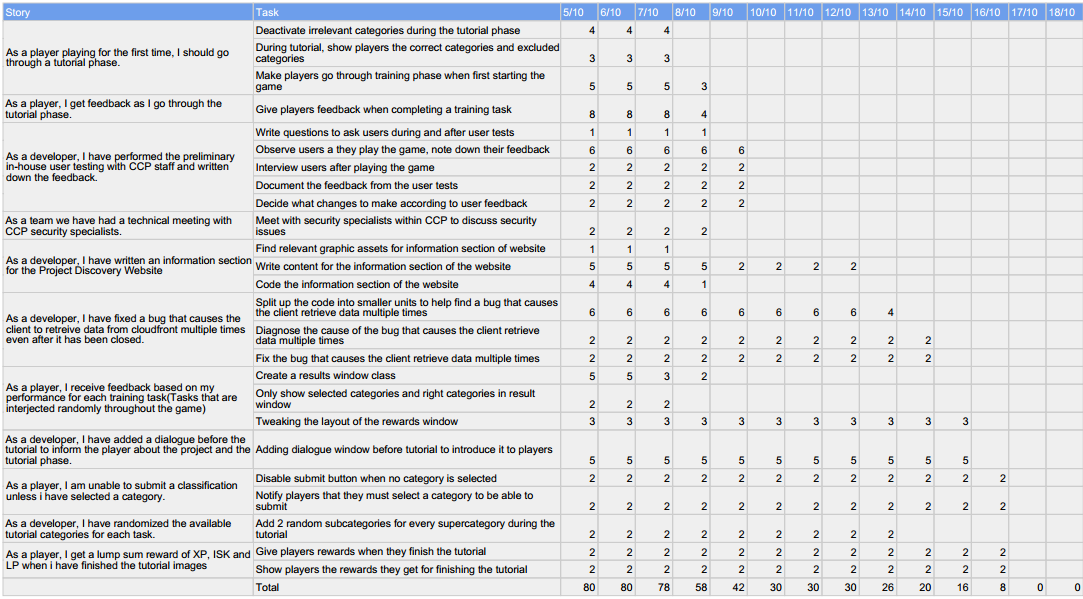
\includegraphics[scale=0.7]{sprint4.PNG}}
    \caption{\label{fig:s4}Sprint backlog for sprint 4}
\end{figure}

\end{landscape}

\begin{figure}[H]
	\centering
	\graphicspath{ {./graphics/} }
    \centerline{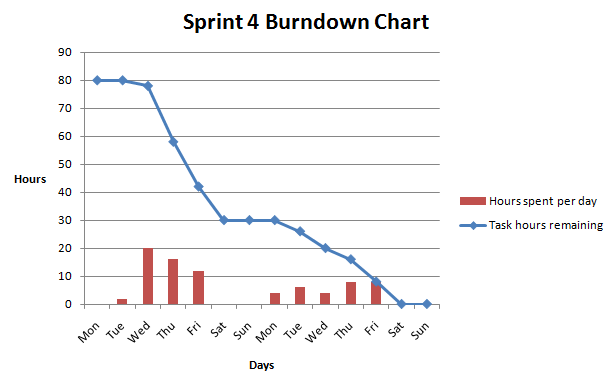
\includegraphics[scale=0.8]{sprint4bdc.PNG}}
    \caption{\label{fig:s4bd}Sprint burndown chart for sprint 4}
\end{figure}